
\begin{minipage}[c]{\textwidth}
\centering
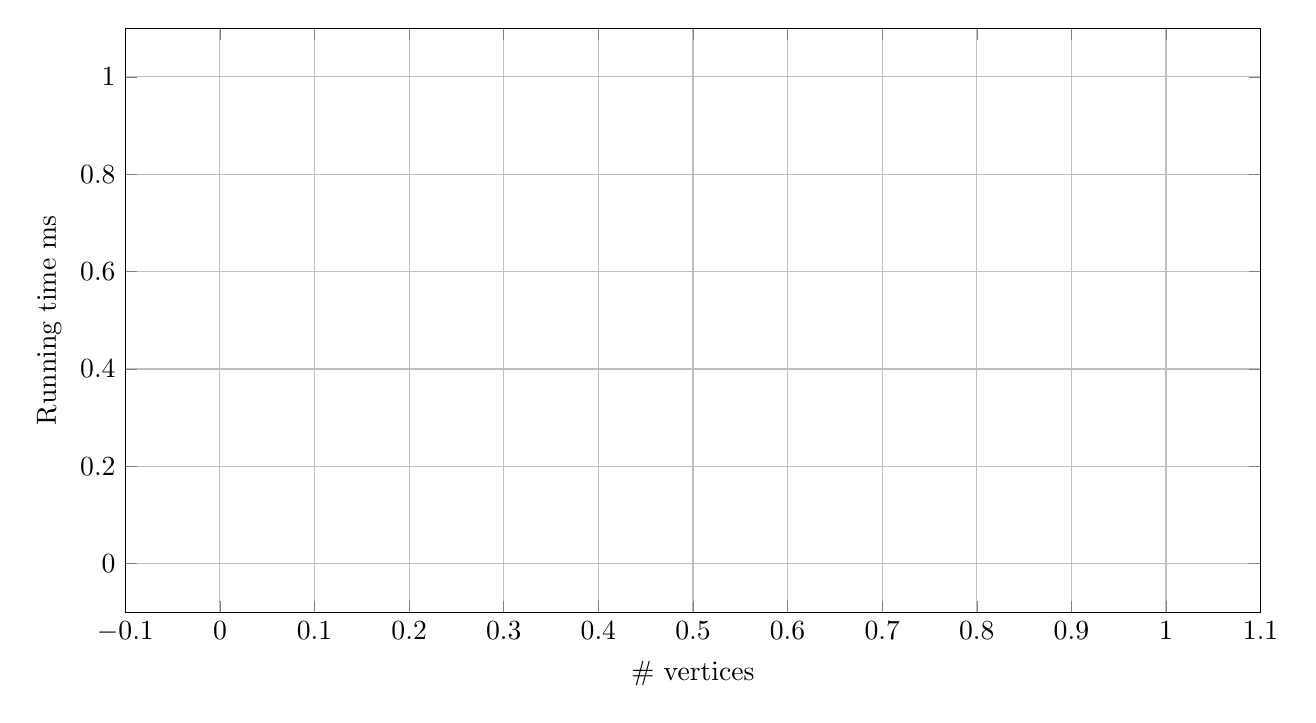
\begin{tikzpicture}
        \begin{axis}[
            xlabel = \# vertices,
            ylabel = Running time ms,
            height=9cm,
            width=16cm,
        	grid=major,
            legend pos=north west
    	]
    		
    	\addplot coordinates {
    	};
        
    	\addlegendentry{\textsc{djk1-bha}}

                \addplot coordinates {
    	};
        
    	\addlegendentry{\textsc{djk1-bhp}}

        \addplot coordinates {
    	};
        
    	\addlegendentry{\textsc{djk1-fh1}}

        \addplot coordinates {
    	};
        
    	\addlegendentry{\textsc{djk1-fh2}}


        \addplot coordinates {
        };
        
    	\addlegendentry{\textsc{djk2-bha}}

        \addplot coordinates {
        };
        
        \addlegendentry{\textsc{djk2-bhp}}

        \addplot coordinates {
        };
        
        \addlegendentry{\textsc{djk2-fh1}}
        
        \addplot coordinates {
        };
        
        \addlegendentry{\textsc{djk2-fh2}}

        \end{axis}

    \end{tikzpicture}
    \captionof{figure}{Average time of running \textsc{Dijkstra1} and \textsc{Dijkstra2}}
    \label{fig:sample_figure}
\end{minipage}